\documentclass{beamer}
\usecolortheme{dolphin}
\usepackage{graphics}
\usepackage{graphicx}
\usepackage{amsmath}
\usepackage{fancyvrb}
\usepackage{color}
\usepackage[ascii]{inputenc}

\title{Writing the Viterbi Algorithm in PyCUDA for CPM decoding}
\subtitle{Project Presentation}
\author{Jon Klein}
\institute{University of Alaska, Fairbanks}
\date{December 7, 2011}

\begin{document}
    \begin{frame}
        \titlepage
    \end{frame}

    \begin{frame}
        \frametitle{Pyterbi is a parallelize Viterbi algorithim written in Python}
        Something here.
        \begin{itemize}
            \item convenient memory allocation and matrix operations 
            \item automatic error checking
            \item automatic object cleanup
        \end{itemize}
    \end{frame}
 
    \begin{frame}
        \frametitle{The Viterbi Algorithm}
        The Viterbi algorithm finds the most likely sequence of states given the outputs.
        It is used for pattern recognition, error-correcting codes, and detecting signals with memory [1].

        \begin{figure}
            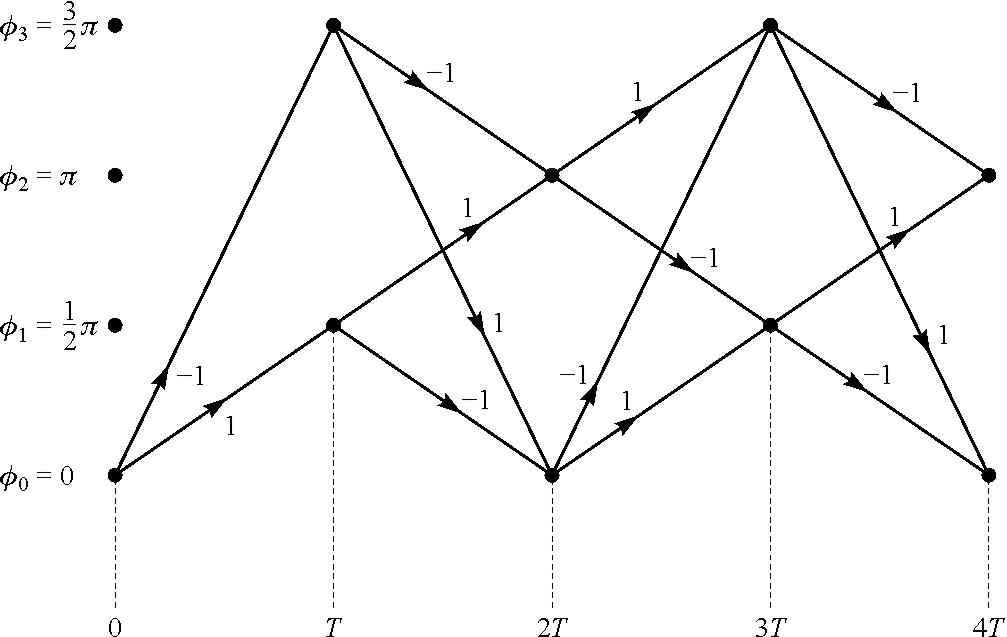
\includegraphics[options]{figures/cpmfulltrellis.jpg}
            \caption{Trellis diagram of $\frac{\pi}{2}$ full response CPM [2]}
        \end{figure}

    \end{frame}
    
    \begin{frame}
        \frametitle{The Viterbi algorithm is parallelizable}
        
        \begin{itemize}
            \item The path leading to a state depends on calculating the path to previous states. The probability of each state at a moment in time can be calculated in parallel.
            \item The Viterbi algorithm can be run on multiple sequences in parallel.
            \item Many of the inputs are constant between between iterations, and can be left on device memory.

        \end{itemize} 
    \end{frame}
    
    \begin{frame}
        \frametitle{The probability of each state depends only on path states}
        \begin{figure}
            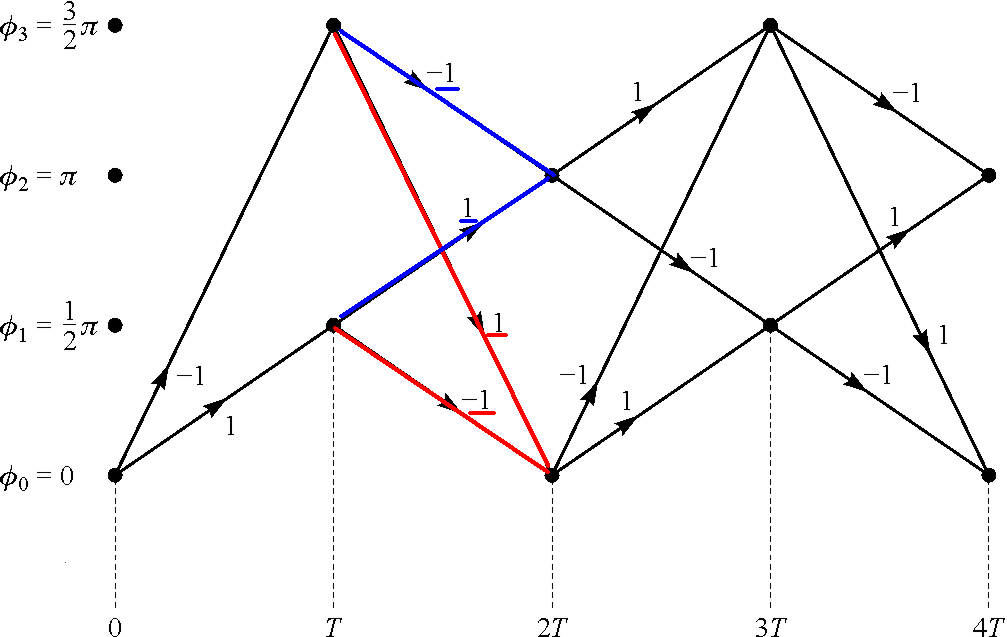
\includegraphics[width=.8\textwidth]{figures/cpmfulltrelliscolored.png}
            \caption{Decoding trellis diagram at time T=2Ts}
        \end{figure}
    \end{frame}
   
    \begin{frame}
    \frametitle{I tried several ways of optimizing the CUDA algorithm..}
    \begin{itemize}
        \item Moving constant matricies from global to constant memory pause slows down execution time by 50\%
        \item Moving less than 8kB of data to constant memory speeds up execution time by 5\%
        \item Moving remaining matricies to shared memory speeds up execution time by another 5\%
        \item Reducing communication between the host and devices provides a ~120\% speedup.
        \item Discarding intermediate values of probability matrix reduces shared memory consumption, permitting more states or longer observation periods.
    \end{itemize}
    \end{frame}

     
    \begin{frame}
        \frametitle{CUDA parallelized pyterbi is at least an order of magnitude faster than the host}
        \begin{figure}
            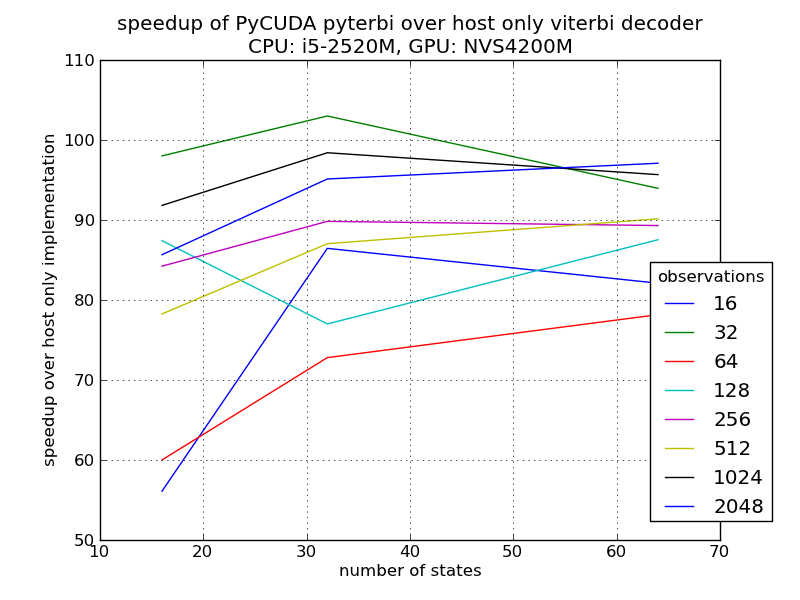
\includegraphics[width=.8\textwidth]{figures/speedupgraphcuda.png}
            \caption{Speedup from parallelizing viterbi algorithm using CUDA}
        \end{figure}

    \end{frame}
    


    \begin{frame}
        \frametitle{SMP parallelized pyterbi will speedup sufficently complex workloads}
        Pyterbi uses the pp Python library to parallize pyterbi by splitting trellises across multiple cores. 
        \begin{figure}
            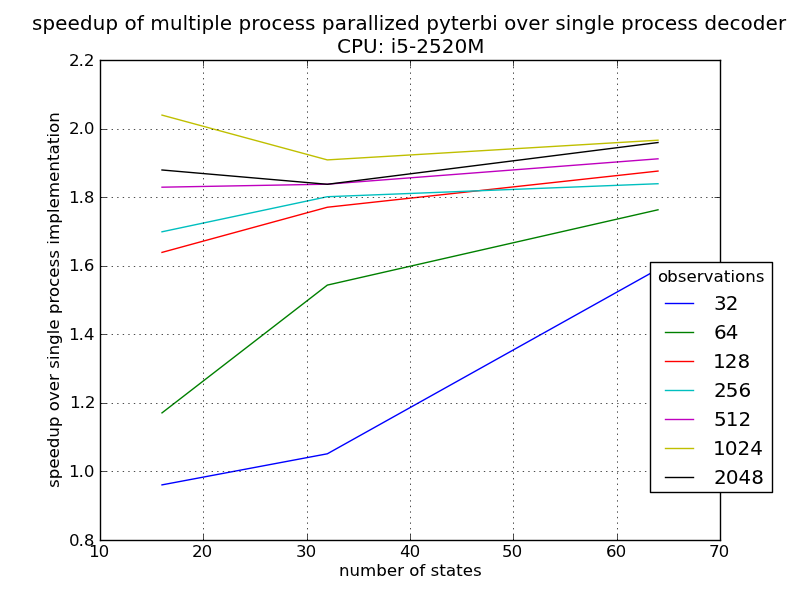
\includegraphics[width=.8\textwidth]{figures/speedupgraphhost.png}
            \caption{Speedup from parallelizing viterbi algorithm using SMP}
        \end{figure}

    \end{frame}
    

    \begin{frame}
        \frametitle{Cluster parallelized Viterbi works, but currently doesn't make sense..}
        
        The pp parallel Python library which pyterbi uses for SMP also works for computer clusters.
        In this mode, the host computer dispatches trellises to an arbitrary number of pp server nodes. 
        
        \begin{columns}[t]
            \begin{column}[t]{.5\linewidth}
            \begin{block}{Node 1}
            \begin{itemize}
                \item Intel i5-2520M, 2.50GHz
                \item 4096MB RAM
                \item Tethered on AT\&T Cell Phone
                \item Ubuntu 11.04
                \item Fairbanks, Alaska
            \end{itemize}
            \end{block}
            \end{column}
            
            \begin{column}[t]{.5\linewidth}
            \begin{block}{Node 2}
            \begin{itemize}
                \item Shared 2.00 GHz AMD Opteron
                \item 192MB RAM
                \item 5 MBps Uplink
                \item Ubuntu 11.04
                \item VPS in New Jersey
            \end{itemize}
            \end{block}
            \end{column}
        \end{columns}
    \end{frame}

    \begin{frame}
        \frametitle{Project Results}
        I have written, tested, and benchmarked:
        \begin{itemize}
            \item a reference host-only implementation of the Viterbi algorithm in Python. 
            \item a CUDA parallelized Viterbi algorithm.
            \item a multi-process and cluster parallelized Viterbi implementation 
        \end{itemize}

        The pyterbi source code is available at: \texttt{http://github.com/loxodes/pyterbi}
   \end{frame}

   \begin{frame}
        There are some possible improvements remaining for pyterbi:
        \begin{itemize}
            \item Rewrite host code in a faster language (C)
            \item Rewrite host code for finer-grained parallelism
            \item Test kernel concurrency on more powerful graphics cards 
            \item Test realistic cases of cluster computing
            \item Get pycuda working with pp for CUDA accelerated cluster computations
        \end{itemize}
    \end{frame}

    \begin{frame}
        \frametitle{References}
        \begin{enumerate}
            \item Lou, H.-L.; , ``Implementing the Viterbi algorithm,'' Signal Processing Magazine, IEEE , vol.12, no.5, pp.42-52, Sep 1995
            \item John Proakis. Digital Communications. McGraw-Hill Science/Engineering/Math, 5 edition, 2007.
            \item C. Liu, ``CuHMM: a CUDA Implementation of Hidden Markov Model Training and Classification,'' 2009 
        \end{enumerate}
    \end{frame}
\end{document}
